\chapter{Nós e Utilizadores}
\label{chap:users} 
%The description of all contacts with users and the results and consequences from such contacts. This includes:
%
%    Interviews and surveys
%    Cultural probes
%    Workshops
%    Usability tests
%    Any other contacts with the users
\section{Entrevistas e Questionários}

No primeiro contacto com o grupo de foco fizemos um pequeno questionário para perceber o quanto conhecem a Cloud e com que regularidade costumam usar e os principais usos.

Com este questionário foi possível concluir que os seguintes factos sobre o grupo de foco:
\begin{itemize}
\item Apesar de usarem a Cloud, ou \textbf{não o que é} ou \textbf{não sabem que usam}. 
\item Usam regularmente a Internet, maioritariamente para o uso de redes sociais e para trocar de emails.
\item Grande parte do grupo também tem o hábito de realizar compras online.
\item Todos os elementos do grupo jogam algum tipo de jogo pelo menos 1 dia por semana.
\item Jogos Multi-jogadores são a preferência da maior parte do grupo.
\end{itemize}

Também tentámos ver como é que estes gostariam de ver um jogo incorporado numa aula, os resultados mostraram que não é aconselhado fazê-lo (Ver Secção \ref{sec:work} para mais informações sobre o tema).

É possível ver o questionário aqui: \url{https://docs.google.com/forms/d/1DeAcM4RT-UcsmGJDCxZHTri0qQV25WQ3CO3uBJQrkNM/viewform}

\section{Cultural Probes}

\begin{figure}[ht]
\centering
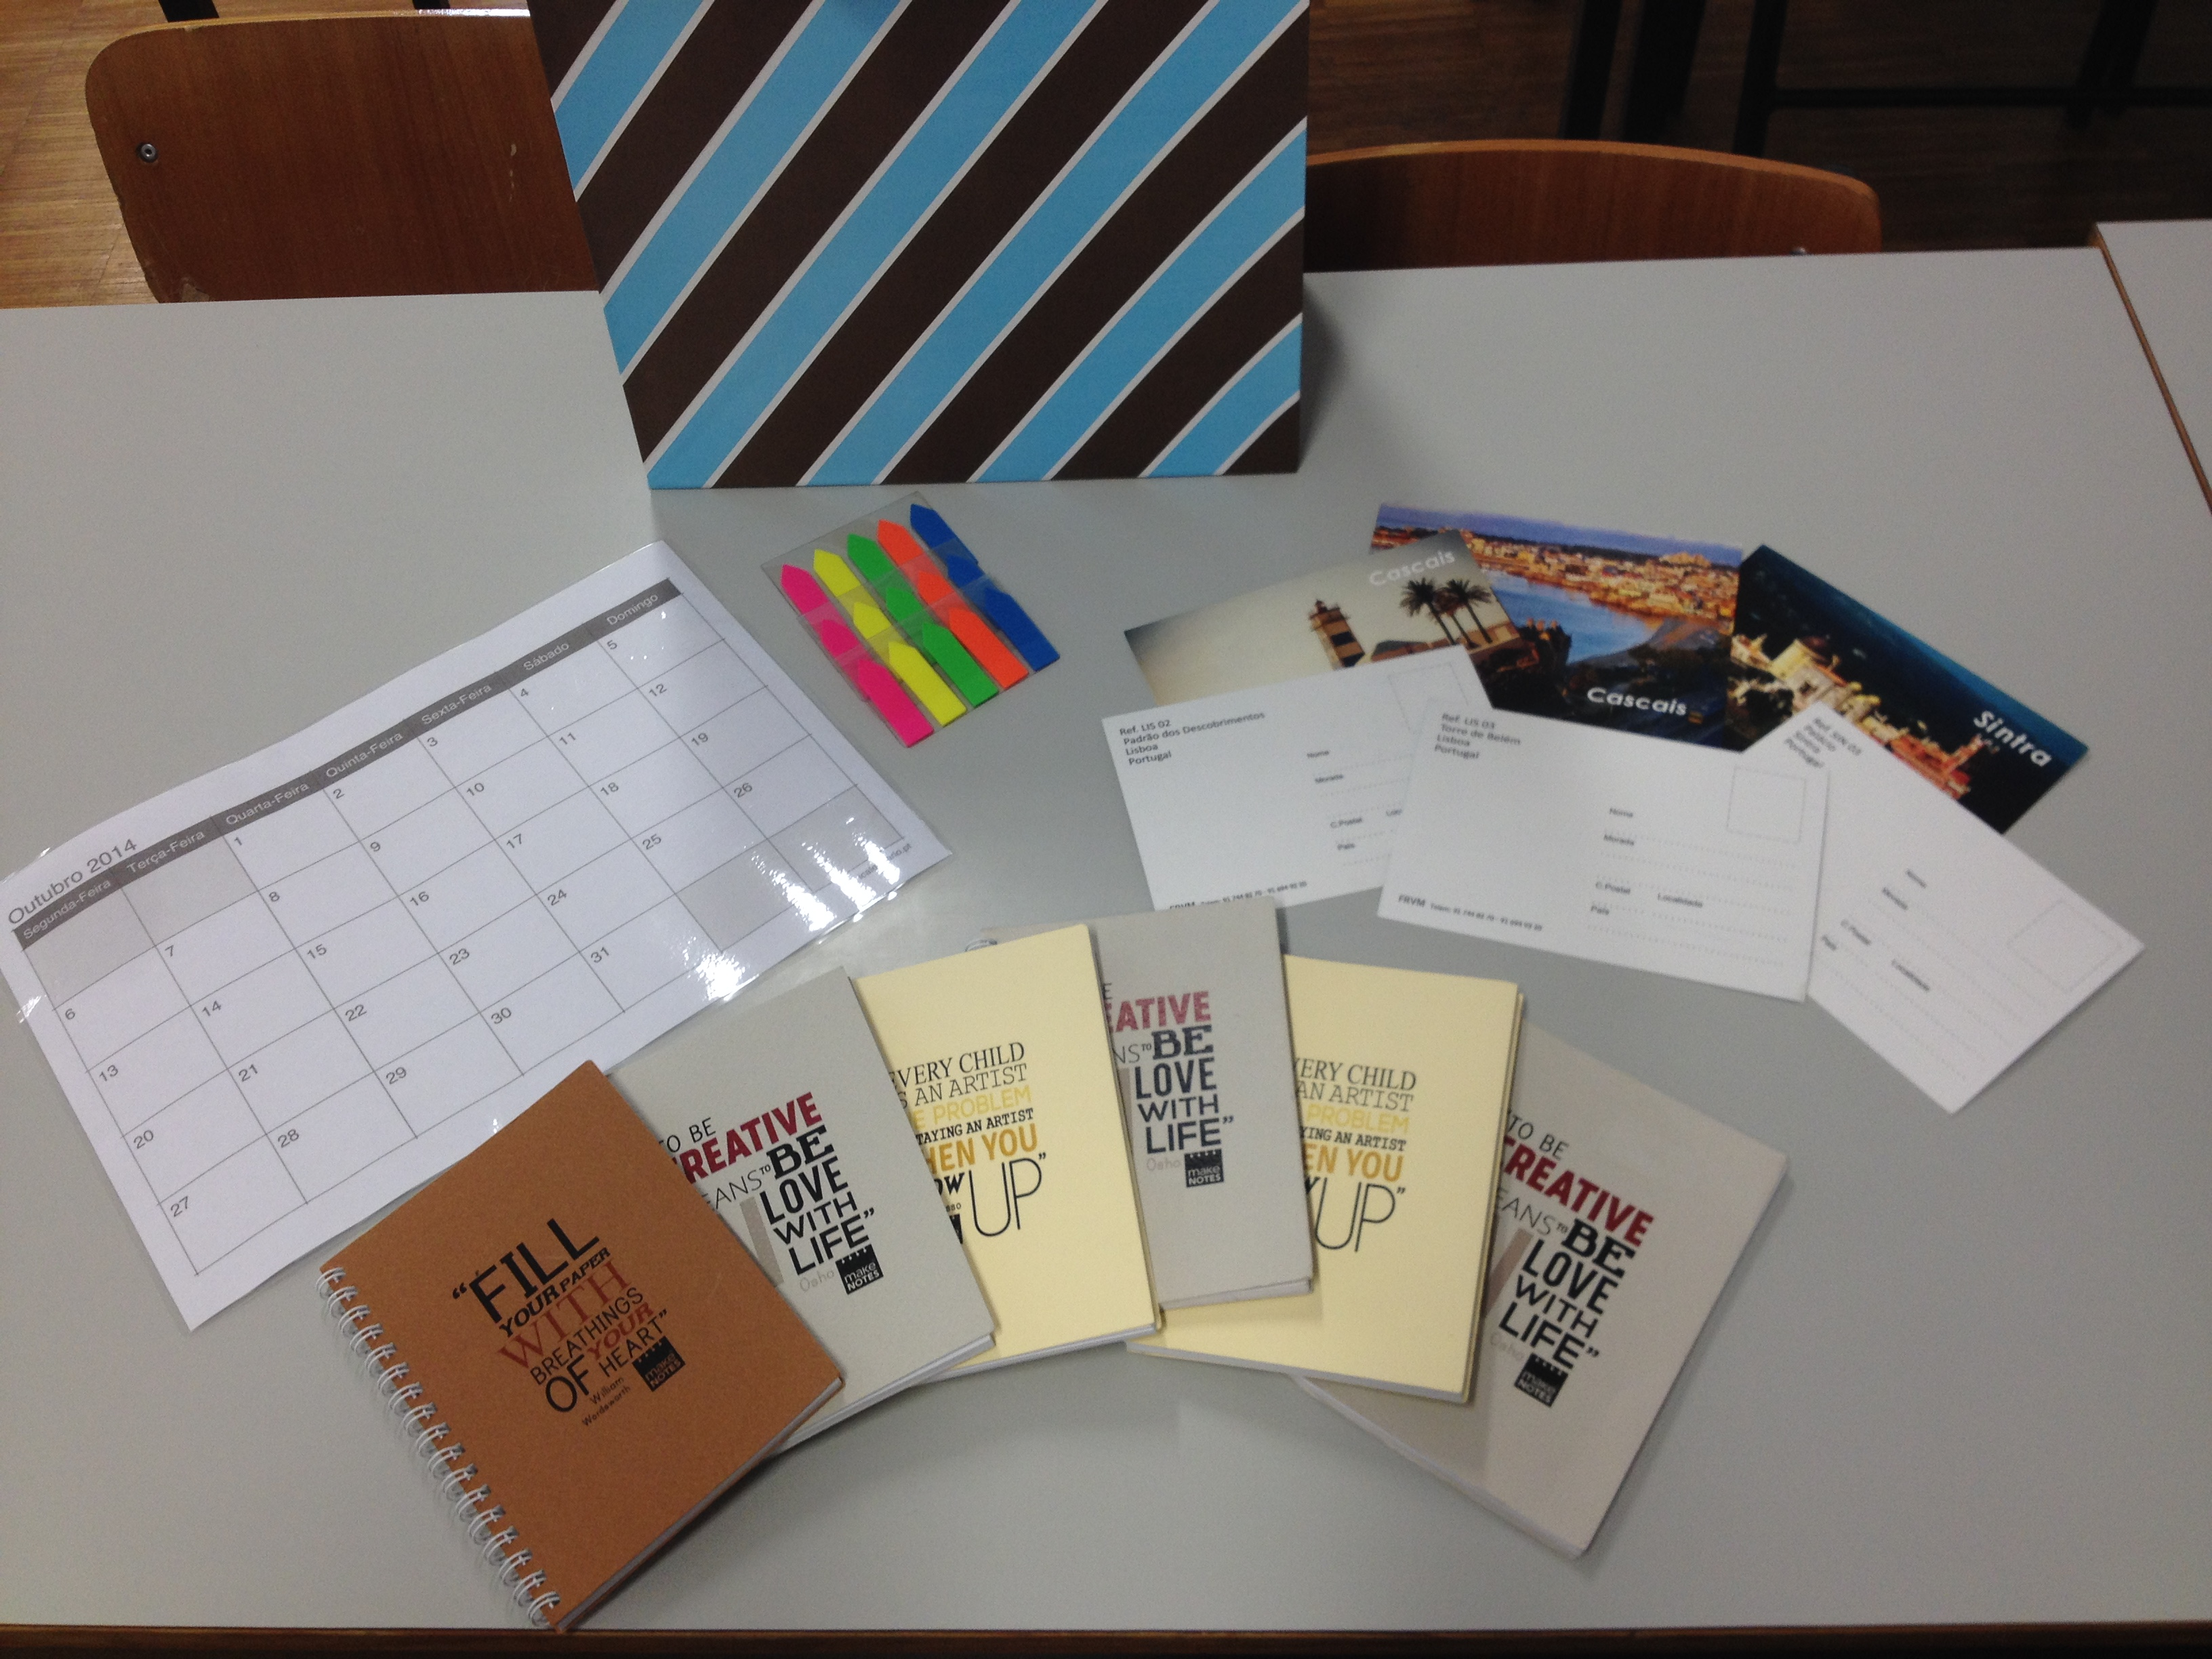
\includegraphics 
	[width = \textwidth] {CulturalProbe}
\caption{\label{fig:probes}} Vista Geral de uma usada Cultural Probes
\end{figure}

As Cultural Probes (Figura \ref{fig:probes}) foram usadas para conhecer melhor alguns hábitos do nosso grupo de foco. Cada uma das Probes continha várias actividades:
\begin{itemize}
\item Um \textbf{calendário} de um mês para ser preenchidos com autocolantes para cada tipo de actividade por dia na Internet (social, jogos, ficheiros, etc.);
\item Um \textbf{diário} para ir escrevendo situações interessantes que vão ocorrendo durante o uso da Internet;
\item \textbf{Postais} com perguntas sobre gostos e opiniões sobre a Internet;
\end{itemize}

Com o calendário concluímos que o uso da Internet para visita de redes Sociais e Email é realizado por aos fins-de-semana, enquanto que videojogos são jogados nas folgas das aulas durante a semana.

Os postais e os diários permitiram concluir que a maior parte do grupo considera a Internet perigosa, não devido a Malwares que possam existir, mas sim pelo número de pessoas que existem Online a qualquer momento do dia, temendo serem espiados.

\section{Workshops}
\label{sec:work}

Para o workshop com o grupo de foco decidimos realizar o Six Thinking Hats sobre como o jogo seria, e o que era necessário para o jogo ser divertido.

O workshop foi realizado com 3 estudantes e não correu como esperado. Os alunos em vez de achar os chapéus interessantes, reagiram com receio de embaraço. A adopção de uma conversa aberta sobre o tema permitiu a recolha da informação pretendida.

Com este chegamos à conclusão que um jogo apenas de perguntas e respostas não traria o interesse desejado ao grupo, e que um jogo de aventura seria mais apelativo, como por exemplo um jogo com história e pistas. Reparamos também que os utilizadores gostam bastante de jogos de competição e comparar resultados.

Para além disto notámos que nem todos os alunos têm um smartphone nem tablet, mas que a maior parte possui um portátil, mesmo que não seja topo de gama.
A maior parte dos alunos deram a entender que o jogo deve ser simples mas ter conteúdo relevante e actividades não monótonas.

Também concluímos que a aplicação de um videojogo num sala de aula no secundário é uma má escolha, pois será usado poucas vezes e seria monótono e pouco divertido, para além de acarretar todo o custo que a preparação de uma aula implica.

Originalmente o workshop foi planeado tendo também uma actividade de PICTIVE onde o grupo iria desenhar uma possível interface para o jogo que eles gostariam de jogar, mas esta actividade teve de ser excluída por falta de disponibilidade dos alunos.

\section{Outras Actividades}
Para além das restantes actividades criámos um grupo no Facebook\footnote{O grupo criado é privado, não sendo assim partilhadas quaisquer imagens deste.} onde contactávamos com o grupo de foco e partilhávamos posts engraçados e experiências na Internet.

Este grupo permitiu criar uma ligação mais próxima entre todos os elementos e facilitou a marcação de reuniões.